\documentclass[letterpaper,12pt]{article}

\usepackage{setspace}
\onehalfspacing

% waste less space around section titles etc.
\usepackage{titlesec}
\titlespacing*{\section}
{0pt}{1ex}{0.65ex}%{0pt}{1.5ex}{0.75ex}
\titlespacing*{\subsection}
{0pt}{0.9ex}{0.4ex}%{0pt}{1ex}{0.5ex}
\titlespacing*{\subsubsection}
{0pt}{0.7ex}{0ex}%{0pt}{0.75ex}{0ex}
\titlespacing*{\paragraph}
{0pt}{0.7ex}{1em}%{0pt}{0.75ex}{1em}

\usepackage[margin=1in]{geometry}
\usepackage{pdfpages}
\usepackage{microtype}
\usepackage{wrapfig}
\usepackage{subcaption}
\usepackage{amsmath,amssymb,amsthm}
\usepackage{hyperref}
\usepackage{array}
\usepackage{booktabs,url}
\usepackage{color}
\usepackage{afterpage}
\usepackage{enumitem}
\usepackage{times,psfrag,epsf,epsfig,graphics,graphicx}
\usepackage{algorithm}
\usepackage{algorithmic}
\usepackage{fancyvrb}
\usepackage{tikz}
\usepackage{cite}

%%%%%%%%%%%%%%%%% actual document starts here

\title{Using Tangly Statistics to Truncate Blockchain Growth}

% change these to what applies
\author{Nathan Stouffer advised by Dr. Mike Wittie}
\date{}

\begin{document}

\maketitle

\documentclass[11pt]{article}

\usepackage[margin=1in]{geometry}
\usepackage{titlesec}
\usepackage{enumitem}
\usepackage{amssymb,amsmath}
\usepackage{times,psfrag,epsf,epsfig,graphics,graphicx}
\usepackage{algorithm}
\usepackage{algorithmic}
\usepackage{tikz}

\title{Capstone Abstract}
\author{Nathan Stouffer}
\date{}

\begin{document}
    \maketitle

    % blockchains are interesting and useful
    Blockchains provide a way to decentralize ledger-keeping systems.
    They are best known for their use in cryptocurrencies, but blockchains also have applications in supply chain tracking, providing data integrity, and any situation where information needs to be immutable.
    To provide immutability, blockchains use Proof of Work to construct an ever growing chain of blocks in a peer to peer network.
    Miners are expected to expend computational work to create a new block.
    Since blocks are intetionally difficult to create, users of a blockchain can trust the information held in the longest blockchain.

    % problem with blockchains
    Miners technically have complete control over a blockchain, but if the miners are sufficiently decentralized, they cannot make a substantial impact on the blockchain by deviating from the protocol.
    Thus a blockchains perform better when control of the chain is decentralized.
    However, decentralized mining can become difficult to achieve when blockchains grow to an unmanageable length.
    To begin mining, one must download and process the entire chain.
    For Bitcoin (the most popular blockchain), it can take days to become a full fledged miner.
    This decreases decentralization in two ways.
    First, lightweight devices are prevented from becoming miners.
    Even desktops and laptops will soon not be able to become a Bitcoin miner.
    Second, people are less likely to become a miner because of the incredibly long bootstrapping time.
    Together, these issues decrease decentralization in a blockchain which reduces the effectiveness of a blockchain.

    % idea for a solution

    % implementation

    % expected results

\end{document}


\section{Introduction}
\label{sec:introduction}

% >> This needs to tell a story: big picture problem, identify a "shortcoming", narrow it down to a specific gap that you are going to address.

% societal problem
% technical problem
% technical solution
% expected impact

Blockchain was introduced in order to provide distributed consensus without relying on a central party~\cite{nakamoto2009Bitcoin}.
Avoiding a central party provides two benefits.
First, there is no central location that an attacker can access to compromise a system.
A centralized blockchain is much easier to compromise than a decentralized blockchain.
Second, there is no single party with complete control over a system.
An example of where decentralized control is useful is in international currency exchange.
Banks have the power to charge high transaction fees for international monetary transfers and customers are forced to pay the fees because there is no alternative.
Legitimate cryptocurrencies have enough competition between parties (miners) that there is no room for a monopoly, giving customers a cheaper option.

Bitcoin was released to the general public in 2009 as the first implementation of a blockchain.
Bitcoin garnered a lot of support and quickly became one of the most prominent cryptocurrencies.
Since Bitcoin's inception, blockchains have found other applications.
They are used in other cryptocurrencies, verify supply chains, and increase device autonomy in the Internet of Things~\cite{cai2018DecentralizedApplications}.
Blockchains are even being used to provide security and privacy in the medical field~\cite{siyal2019MedicalApplications}.
Blockchain technology has the potential to enhance data security in a wide range of diverse applications.

Blockchain’s services are best realized when control of the chain is decentralized.
Decentralized control can become difficult to achieve when blockchains grow to an unmanageable size.
I am writing this proposal to request funding to work on a method to truncate  blockchains.
My work on this project will be a continuation from the REU research I collaborated on this summer.
We have a solution sketch and a prototype implementation, but more work needs to be done to prove the correctness of the solution and to translate the prototype to a practical implementation.
If successful, this project has the possibility of making blockchains more effective, extending data reliability and user privacy~\cite{cai2018DecentralizedApplications}~\cite{siyal2019MedicalApplications}.

The remaining sections provide information regarding background information, my plan, an estimated time line, and other logistical details.


\includepdf[pages=-]{resume.pdf}

\section{Background}
\label{sec:background}

\subsection{Blockchain}

At a high level, a blockchain is a sequence of blocks that is immutable in practical applications.
Immutability in blockchains is often provided through Proof of Work.
Proof of Work was introduced in \cite{dwork1992PoW} and first used for blockchain in the Bitcoin whitepaper \cite{nakamoto2009Bitcoin}.
In a Proof of Work blockchain, a block is valid if its cryptographic hash is below a preset threshold.
Each block primarily consists of data that cannot change (financial transactions, medical records, etc).
However, every block contains a field for a fixed-length string of bits that make the output of the hash function below the threshold.
The fixed-length string is called a nonce.
If someone finds a nonce, they have ``mined'' a block.
Since the hash function is cryptographic, it is difficult to reverse.
The best strategy for someone mining a block is to guess and check nonces until a sufficiently low output is found.
Figure \ref{fig:blockchain} displays the typical structure of a blockchain.

\begin{center}
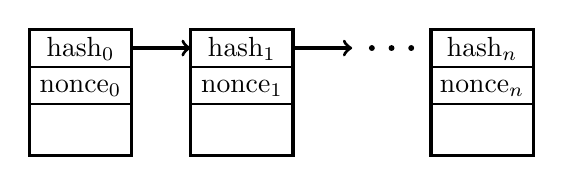
\begin{tikzpicture}[scale=1]

% drawing block 0
\draw [very thick] (0.0,0) rectangle (1.3,1.6);
\draw [white] (0.65,1.35) circle (0.01) node[text=black] {hash$_0$};
\draw [thick] (0.0,1.125) -- (1.3,1.125);
\draw [white] (0.65,0.8500000000000001) circle (0.01) node[text=black] {nonce$_0$};
\draw [thick] (0.0,0.6500000000000001) -- (1.3,0.6500000000000001);
% drawing arrow
\draw [->, very thick] (1.3,1.3625) -- (2.05,1.3625);

% drawing block 1
\draw [very thick] (2.05,0) rectangle (3.3499999999999996,1.6);
\draw [white] (2.6999999999999997,1.35) circle (0.01) node[text=black] {hash$_1$};
\draw [thick] (2.05,1.125) -- (3.3499999999999996,1.125);
\draw [white] (2.6999999999999997,0.8500000000000001) circle (0.01) node[text=black] {nonce$_1$};
\draw [thick] (2.05,0.6500000000000001) -- (3.3499999999999996,0.6500000000000001);
% drawing arrow
\draw [->, very thick] (3.3499999999999996,1.3625) -- (4.1,1.3625);

% draw the dots
\draw [fill=black] (4.35,1.3625) circle (0.03);
\draw [fill=black] (4.6,1.3625) circle (0.03);
\draw [fill=black] (4.85,1.3625) circle (0.03);

% drawing block n
\draw [very thick] (5.1,0) rectangle (6.3999999999999995,1.6);
\draw [white] (5.75,1.35) circle (0.01) node[text=black] {hash$_n$};
\draw [thick] (5.1,1.125) -- (6.3999999999999995,1.125);
\draw [white] (5.75,0.8500000000000001) circle (0.01) node[text=black] {nonce$_n$};
\draw [thick] (5.1,0.6500000000000001) -- (6.3999999999999995,0.6500000000000001);

\end{tikzpicture}
\end{center}

A broader perspective of a blockchain is an implementation of a finite state machine.
In the state machine, blocks are transitions between the states of applications running on top of a blockchain.
Abstractly, the $k^{th}$ block $B_k$ is a transition from state $S_{k-1}$ to state $S_k$ with certain validity requirements.
See Figure \ref{fig:statemachine} for a visual.
A tangible example is a cryptocurrency.
Cryptocurrencies realize state as a record of the amount of currency each public key controls.
Blocks are a set of transactions that transfer currency between public keys.
In state $S_0$, no one controls any currency.
Then block $B_1$ moves the blockchain to $S_1$ where its miner controls some newly created currency.
Then block $B_2$ grants cryptocurrency to its miner and contains currency transfers between users of the currency.
This process repeats until state $S_n$ is reached, which contains the current account-balance pairs of all the current users of a cryptocurrency.

\begin{center}
    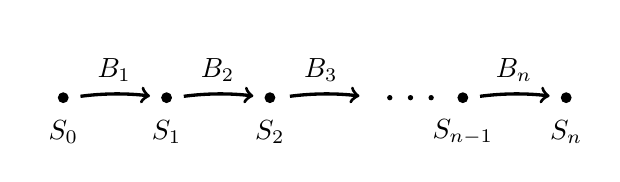
\begin{tikzpicture}[scale=1.75]
        % draw the 0 point
        \draw [thick,color=white] (0,0) -- (0,0);

        % state 0
        \draw [fill=black] (0.25,-0.5) circle (0.035);
        \node at (0.25,-0.75) {$S_0$};

        % block 1
        \draw [very thick, ->] (0.375,-0.49) arc (97.5:83:2);
        \node at (0.62,-0.3) {$B_1$};

        % state 1
        \draw [fill=black] (1,-0.5) circle (0.035);
        \node at (1,-0.75) {$S_1$};

        % block 2
        \draw [very thick, ->] (1.125,-0.49) arc (97.5:83:2);
        \node at (1.37,-0.3) {$B_2$};

        % state 2
        \draw [fill=black] (1.75,-0.5) circle (0.035);
        \node at (1.75,-0.75) {$S_2$};

        % block 3
        \draw [very thick, ->] (1.895,-0.49) arc (97.5:83:2);
        \node at (2.12,-0.3) {$B_3$};

        % ...
        \draw [fill=black] (2.62,-0.5) circle (0.015);
        \draw [fill=black] (2.77,-0.5) circle (0.015);
        \draw [fill=black] (2.92,-0.5) circle (0.015);

        % state n-1
        \draw [fill=black] (3.15,-0.5) circle (0.035);
        \node at (3.15,-0.75) {$S_{n-1}$};

        % block n
        \draw [very thick, ->] (3.275,-0.49) arc (97.5:83:2);
        \node at (3.52,-0.3) {$B_n$};

        % state n
        \draw [fill=black] (3.90,-0.5) circle (0.035);
        \node at (3.90,-0.75) {$S_n$};

    \end{tikzpicture}
    \captionof{figure}{Blocks as transitions between states \label{fig:statemachine}}
\end{center}


\subsection{Technical Problem}

To understand the technical problem, we must understand two properties of blockchains.
First, we observe that miners must have every block in the chain to contribute new blocks.
And, second, blockchains grow in perpetuity.
These properties mean that new miners must download and process an ever increasing amount of data as time passes.
Even now, when Bitcoin is just over a decade old, it can take days or weeks to become a miner.
Such a barrier prevents some nodes from mining, limiting decentralization.
Less decentralization reduces the effectiveness of a blockchain.

When viewing a blockchain as a finite state machine, we can change the requirements of what a miner needs to know.
All a miner must know is a state $S_k$ and every block following that state.
Then a bootstrapping miner could compute the current state.
If $S_k$ is close to the end of the chain, then the miner requires significantly less bootstrapping time by only requesting blocks following $S_k$.

How does a bootstrapping miner obtain the state $S_k$?
They can't just ask a blockchain node, because they could receive a faulty state.
This is the problem we would like to solve: Can we provide a mechanism so that a bootstrapping node can trust a recent state?

\subsection{Related Work}

% lightweight nodes in the bitcoin whitepaper

% summary block in the main chain

% miniblockchain

% separate summary chain

% coinprune 

Our solution gains inspiration from a paper written by Matzutt et al. that provides a way to verify Bitcoin states.
They suggest that recent miners be allowed to vote for a state and then bootstrapping nodes trust the majority of votes.
Each vote is recorded in a block and each block has the capacity to store a single vote \cite{matzutt2020HowTSPrune}.
Storing votes in blocks gives them immutability, so a bootstrapping node knows that they are counting every vote.

There are two problems with this idea.
First, a vote can only be generated as quickly as new blocks.
In Bitcoin, this averages to about 10 minutes per block, meaning a bootstrapping node might have to wait a week for there to be sufficiently many votes to trust a state.
Second, this solution relies on implementation details in the Bitcoin protocol and may not apply to blockchains in general.


\section{Goal}
\label{sec:goal}

\section{Methodology}
\label{sec:methodology}

% provide enough information so that someone can replicate

Much of this project is devising a method to bootstrap blockchain nodes.
Since this is a conceptual task, it cannot be replicated.
However, the experimental verification of our protocol can be replicated.
Section \ref{sec:methodology} is devoted to providing the necessary information for someone to replicate our implementation.

% network simulator with dht

In order to match our model as closely as possible with our implementation, we chose to implement our solution on a network simulator using a full-fledged DHT.
This is not strictly necessary but we felt that it made our results more applicable to a real implementation of our idea.

% digitally signed parents

A neglected detail of the solution is the process of selecting parents in the tangle.
The tangle manager has complete control over \textit{which} votes are selected as parents, but we require that the parents are digitally signed in the vote.
This means that the manager must tell the voter which votes are the parents and the voter includes that information in their vote.
While this is some overhead communication for our solution, it prevents a malicious actor from changing the structure of a tangle to their advantage.

% attacker intelligence

The most important aspect of the implementation is the intelligence of the attackers.
We expect the constraints of our solution to prevent an attacker from \textit{successfully} fooling a bootstrapping node.
But the only way we can verify this is to simulate intelligent attackers.
We have divided attacks into two categories: deleting votes and reordering votes.
An accurate replication of this project should at least implement these strategies.
Implementing more strategies is welcome, since it provides more information on our system!

% chi-squared test

We used the $\chi ^2$ test as follows.
Consider some sample of votes $S$ and our expected proportion of agreeing votes $\beta$.
Our distribution comes in the form $(majority, other)$ where $majority$ references the number of valid votes that supported the most popular state and $other$ is the number of valid votes that did not support the most popular state.
We have an expected distribution $(\beta|S|, (1-\beta)|S|)$ and an actual distribution of $(S_{maj}, S_{oth})$.
Then we can use the $\chi ^2$ test to determine the probability that our sample comes from the expected distribution.

\subsection{Design}

\newcommand{\operation}{$+$sortedVotes() : String[]}

\begin{center}
	\vspace{1em}
    \begin{tikzpicture}[scale=0.9]
    % uml figure

    % boxes (w,l) = (5,3)
    \draw [very thick] (6,6) rectangle (11,9);
    \node at (8.5,8.5) {IVoteSorter};
    \draw [thick] (6,8) -- (11,8);
    \node at (8.5,7.65) {\operation};

    \draw [very thick] (0,0) rectangle (5,3);
    \node at (2.5,2.5) {RndSorter};
    \draw [thick] (0,2) -- (5,2);
    \node at (2.5,1.65) {\operation};

    \draw [very thick] (6,0) rectangle (11,3);
    \node at (8.5,2.5) {BFSSorter};
    \draw [thick] (6,2) -- (11,2);
    \node at (8.5,1.65) {\operation};

    \draw [very thick] (12,0) rectangle (17,3);
    \node at (14.5,2.5) {DescSorter};
    \draw [thick] (12,2) -- (17,2);
    \node at (14.5,1.65) {\operation};

    % lines
    \draw [dashed, -{Triangle[open, width=3.5mm, length=3mm]}] (8.5,3) to (8.5,6);
    %\draw [dashed, very thick] (6.5,3) -- (6.5,5.7);
    \draw [dashed, very thick] (2.5,3) -- (2.5,4);
    \draw [dashed, very thick] (2.5,4) -- (6.5,4);
    \draw [dashed, very thick] (14.5,3) -- (14.5,4);
    \draw [dashed, very thick] (14.5,4) -- (6.5,4);

    \end{tikzpicture}
    \captionof{figure}{Strategy Pattern for vote sorters\label{fig:strategy}}
\end{center}



\section{Results}
\label{sec:results}

% this section must be devoid of opinion

% Q1: is the solution off-chain?
% M1: number of changes to the blockchain protocol

% Q2: is the solution efficient?
% M2: asymptotic analysis of time and space requirements as the chain grows
% M3: bytes of network traffic generated

\begin{center}
\begin{table}[h]
    \centering
    \begin{tabular}{|l|l|l|l|}
        \hline
                  & Max time & Min time & Average time \\ \hline
        Algorand  & 2149 s   & 758 s    & 939  s       \\ \hline
        Bitcoin   & 1512 s   & 796 s    & 1038 s       \\ \hline
        Ethereum  & 2243 s   & 711 s    & 1108 s       \\ \hline
    \end{tabular}
    \caption{INSERT CAPTION}
    \label{tab:gqm}
\end{table}
\end{center}


% Q3: is the solution secure?
% M4: theoretical probability that a malicious actor fools a bootstrapping node
% M5: empirical probability that a malicious actor fools a bootstrapping node

\begin{figure}[h]
	\centering
	\includegraphics[width=\linewidth]{img/deleter}
	\caption{INSERT CAPTION}
	\label{fig:deleter}
\end{figure}

\begin{figure}[h]
	\centering
	\includegraphics[width=\linewidth]{img/rejecter}
	\caption{INSERT CAPTION}
	\label{fig:rejecter}
\end{figure}

\section{Discussion}
\label{sec:discussion}

% complement results with opinions and reasoning

\section{Conclusion}
\label{sec:conclusion}

% conclude and discuss future work

%%%%%%%%%%%%%%%

\clearpage
%References Cited (include in an additional page within the project proposal): Include a list of any literature that you have cited in the proposal. Nearly all good science and engineering proposals cite papers reporting related results, describing the methods to be used or providing background information. Please note-the review panel rarely recommends funding for proposals without adequate references.

\bibliographystyle{unsrt}
\bibliography{bibliography/refs.bib}
% make sure that there is bibliography.bib file with bibtex references, to be cited above using \cite{bibkey} where bibkey is the label of the reference in bibtex


%%%%%%%%%%%%%%%%
% uncomment and complete the following if it applies

\clearpage

\end{document}
